W artykule opublikowanym przez firmę Microsoft o tytule \enquote{Co to jest cyberbezpieczeństwo ?}~\footnote{Artykuł jest dostępny pod adresem: https://www.microsoft.com/pl-pl/security/business/security-101/what-is-cybersecurity}, trzy z sześciu wymienionych typów zagroże to: 
\begin{itemize}
    \item oprogramowanie wymuszające okup,
    \item inżynieria społeczna,
    \item wyłudzanie informacji.
\end{itemize}
Autorzy prawdopodobnie nie bez powodu nazwali pierwszy z powyższych typów tak, a nie jako \enquote{atak oprogramowaniem wymuszjącym okup}. Atak ransomware zawiera w sobie każde z tych zagrożeń. Oprogramowanie złośliwe wymaga od ofiary zaufania o tym, że oprogramowanie, które uruchamiają, jest nieszkodliwe. Typowo propagacja takiego oprogramowania ma miejsce poprzez tzw. \foreignquote{english}{phishing} czyli podszywanie się atakującego poprzez zaufany serwis lub instytucję, z którym ofiara mogła wejść w interakcję w przeszłości. Aby zrozumieć zakres tych technik oraz możliwe wektory ataku, należy prześledzić ich historię.
%%%%%%%%%%%%%%%%%%%%%%%%%%%%%%%%%%%%%%%%%%%%%%%%
\section{Historia i ewolucja ataków typu ransomware}
\subsection{Wczesna historia}
Mimo stopniowego nasilania się ataków ransomware w przeciągu ostatnich 7 lat sama idea utrudnienia
dostępu do plików pod groźbą okupu jest znana od dosyć dawna. Już w drugiej połowie lat 80-tych, w USA,
cyberprzestępcy w zamian za odzyskanie dostępu do danych wyłudzali okup, który następnie był wysyłany drogą pocztową. Jednym z pierwszych udokumentowanych ataków wirusem ransomware był DOSowy \foreignquote{english}{AIDS trojan}~\cite{virus_1990} z 1989 roku. Autor programu — Joseph Popp — przekazywał dyskietki drogą pocztową do wybranej grupy ofiar pod przykrywką załącznika do ulotki informacyjnej na temat wirusa AIDS. Program modyfikował plik \texttt{AUTOEXEC.BAT}, z którego korzystał w celu zliczenia ilości uruchomień komputera. W momencie przekroczenia liczby 90 uruchomień szyfrował nazwy wszystkich plików na dysku \texttt{C:\/}, tym samym uniemożliwiając korzystanie z systemu.
\begin{figure}[H]
    \centering
    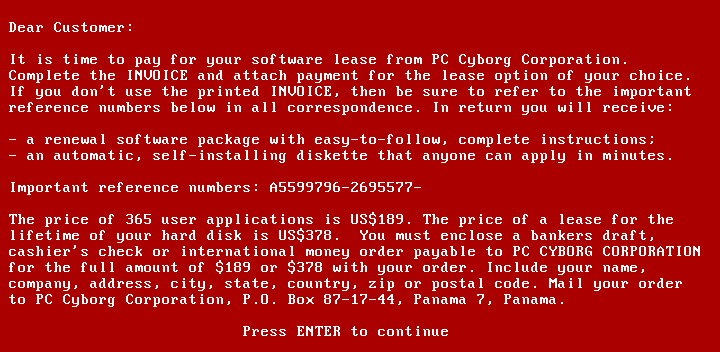
\includegraphics[width=0.6\linewidth]{rysunki/aids-trojan.png}
    \caption{Wiadomość ukazująca się po aktywacji wirusa \foreignquote{english}{AIDS trojan}}
    \label{fig:enter-label}
\end{figure}
Atakujący podszywał się pod fikcyjną korporację \foreignquote{english}{PC Cyborg Corporation}, na której adres w Panamie miał być wysyłany okup. Paczka razem z dyskietką posiadała również ulotkę z krótkim wprowadzeniem, instrukcją obsługi, a także licencją co było w tamtym czasie powszechną i budzącą zaufanie praktyką. 
Program nie szyfrował treści samych plików, jedynie ich nazwy. Klucz szyfrowania był kluczem symetrycznym, co sprawiało, że złamanie go mogło pomóc odblokować system, każdej ofierze borykającej się z tą samą wersją wirusa. Eliminacja tej wady była inspiracją dla pracy \foreignquote{english}{Cryptovirology: Extortion-Based Security Threats and Countermeasures}, w której przedstawiono pojęcie \foreignquote{english}{cryptovirological attack}~\cite{yung}.
\newline
Po roku 1996, w erze upowszechnienia się internetu, pojawiły się sporadyczne ataki ransomware na niewielką skalę, tym razem ulepszone o szyfrowanie hybrydowe. W latach dwutysięcznych pojawił się trudny do wykrycia \foreignquote{english}{PGPCoder}~\cite{tromer_cryptanalysis_nodate} używający 660-bitowego klucza RSA. Inny, ransomware występującym w tamtym czasie był \foreignquote{english}{Archievus} ~\cite{arhiveus}, również używający klucza RSA, w wersji 1024-bitowej, którego tragiczną wadą było używanie tego samego klucza do szyfrowania każdego pliku na każdej zainfekowanej maszynie. Ataki te, aby zainfekować ofiarę, wykorzystywały phishing i podszywały się pod zaufane strony internetowe. 
%%%%%%%%%%%%%%%%%%%%%%%%%%%%%%%%%%%%%%%%%%%%%%%%
\subsection{Historia współczesna}
Mimo historii sięgającej jeszcze lat 80 - tych, ataki ransomware nie były szczególnie powszechne w latach dwutysięcznych. Status quo został zachwiany po upowszechnieniu się kryptowalut, umożliwiających poufną i trudną do wyśledzenia wymianę środków między ofiarą a atakującym. Jednak uzyskanie pieniędzy od ofiar niezaznajomionych z kryptowalutami nie jest proste, dopiero kantory kryptowalut dały cyberprzestępcom możliwość prostego i poufnego wyłudzenia środków. Pierwsza dekada XXI w. był dla cyberprzestępców czasem udoskonalania \foreignquote{english}{scareware} czyli oprogramowania mającego wystraszyć ofiarę na tyle, żeby zapłaciła za dostęp do stacji, bez wyrządzania szczególnej szkody na danych. 
\newline
W 2013 roku w annały historii internetu wszedł Windowsowy wirus \foreignquote{english}{CryptoLocker}. Wykorzystywał on do szyfrowania 2048-bitową parę kluczy RSA, generowaną na osobnym serwerze, a następnie dostarczał klucz publiczny na stację ofiary w celu szyfrowania jej plików~\cite{cryptolockerfaq}. Tym samym ofiara nie miała innej możliwości odzyskania plików niż zapłacić okup wynoszący 300 USD. Wirus dostarczany był jako załącznik w liście elektronicznym oraz przez owiany złą sławą \foreignquote{english}{Gameover ZeuS botnet}~\cite{zeusbot}. Załącznik posiadał w sobie plik \texttt{.zip}, który z kolei zawierał w sobie plik \texttt{.exe}, z ikonką charakterystyczną dla pliku pdf. Atakujący wykorzystywał domyślne zachowanie Windowsa polegające na ukrywaniu rozszerzenia pliku. Następnie wirus podejmował następujące kroki:
\begin{enumerate}
    \item rozpakowywał swoje pliki w ścieżce profilu użytkownika,
    \item dodawał nową pozycję do windowsowego rejestru, który uruchamiał wirus wraz z rozruchem systemu,
    \item pobierał klucz publiczny z jednego z serwerów,
    \item wirus inicjował szyfrowanie plików na zamontowanych dyskach, w tym na dyskach sieciowych,
    \item wyświetla ekran informujący o zdarzeniu i możliwości opłacenia okupu w BTC do 100 godzin od zaszyfrowania.
\end{enumerate}
Po opłaceniu okupu ofiara miała możliwość pobrania programu dekodującego z załadowanym, odpowiednim kluczem prywatnym. Wirus szyfrował jedynie pliki z odpowiednimi rozszerzeniami m.in. pliki AutoCAD czy dokumenty MS Office.
\begin{figure}
    \centering
    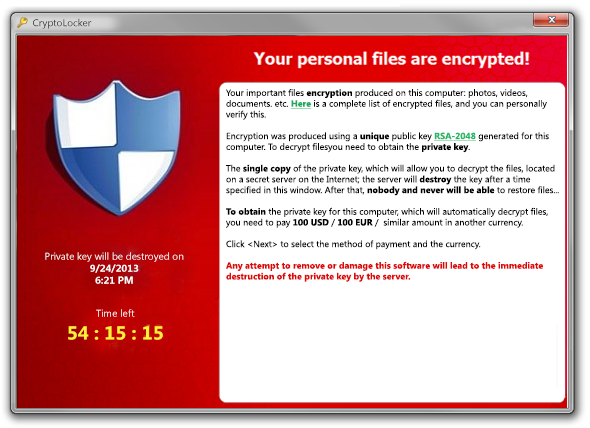
\includegraphics[width=0.75\linewidth]{rysunki/cryptolocker.png}
    \caption{Ekran wyświetlający się po zainfekowaniu komputera przez CryptoLocker.}
    \label{fig:enter-label}
\end{figure}
Zagrożenie zostało zneutralizowane w wyniku zainicjowanej przez departament sprawiedliwości USA, operacji \foreignquote{english}{Tovar}~\cite{tovar} w wyniku której udało się uzyskać dostęp do bazy danych zawierającej prywatne klucze RSA na podstawie których możliwe było odzyskanie plików.
\newline
\foreignquote{english}{CryptoLocker} był swego rodzaju kamieniem milowym w rozwoju cyberprzestępczości. Złożona natura procederu stała się normą dla ataków ransomware a wraz z coraz większą popularnością kryptowalut i usprawnionymi algorytmami szyfrowania asymetrycznego, ilość ataków oraz generowane przez nie straty stabilnie wzrastają aż do dnia dzisiejszego.
\newline
Aktualnie cyberprzestępcy zmienili styl ataku ze skupiającego się na infekcji jak największej ilości stacji, na tzw. \foreignquote{english}{big game hunting}~\footnote{Dokładniejszą definicję z przykładami można znaleźć pod adresem:\newline https://www.malwarebytes.com/blog/news/2023/07/ransomware-making-big-money-through-big-game-hunting}. BGH w dużej mierze polega na koordynacji inżynierii społecznej i zaprojektowania oprogramowania ransomware w sposób, który będzie najbardziej szkodliwy dla dużych organizacji. Obierana jest mniejsza ilość celów na rzecz wyższej kwoty okupu. Raport \foreignquote{english}{CrowdStrike Services} z 2023 roku donosi, że jedną najszerzej stosowanych taktyk BGH jest połączenie ransomware z groźbą upublicznienia skradzionych danych. Typowo dane zostają upubublicznione gdy minie termin zapłaty okupu. Naruszenie danych jest rozłożone w czasie i wykorzystuje narzędzia już dostępne na atakowanym środowisku. Dzięki temu ataki są cięższe do wykrycia~\footnote{Technika ta nosi nazwę \foreignquote{english}{Living off the land}}.
Techniki zastraszenia zostały także dopracowane, aby wywołać możliwie na największą presję na ofiarach. W przypadku \foreignquote{english}{REvil} kradzione dane bywały etapowo upubliczniane, aby zmusić ofiarę do szybszego działania ~\cite{hern_ransomware_2021}.\newline
Z powodu dużej opłacalności takich ataków utworzony został model \foreignquote{english}{ransomware as a service} (RaaS), w którym klienci płacą za dokonanie ataku ransomware programem utworzonym przez inne grupy hakerskie~\footnote{Wykorzystywane jest oprogramowanie utworzone przez inne osoby, podobnie jak w modelu Software as a Service.}. 
\newline
Jednym z nich jest wcześniej wymieniony \foreignquote{english}{REvil} używany przez grupę \foreignquote{english}{PINCHY SPIDER}, którego cechą rozpoznawczą jest postowanie skradzionych danych na blogu \foreignquote{english}{Happy Blog}~\cite{hern_ransomware_2021}. W 2021 roku użyto go na wysoką skalę~\cite{mcmillan_ransomware_2021} przez podatność Kaseya VSA~\footnote{Kaseya VSA jest narzędziem do zarządzania infrastrukturą IT.} o identyfikatorze CVE-2021-30116~\cite{kasaya}. Atak ten można podsumować w następujących krokach:
\begin{enumerate}
    \item użycie komendy \texttt{PowerShell} do zakończenia procesów Windows Defender,
    \item podstawienie pliku wykonywalnego do katalogu instalacyjnego Windowsa,
    \item zgodnie z techniką \foreignquote{english}{Living off the land} wirus pobierał pomocnicze pliki wykonywalne i maskował je nazwami typowymi dla plików pomocniczych Windowsa np. \texttt{agent.exe},
    \item pobrane pliki następnie były przenoszone do odpowiednich folderów w celu załadowania ich razem z plikiem wykonywalnym \texttt{MsMpeng.exe} techniką nazywaną \foreignquote{english}{DLL sideloading}~\footnote{DLL siedloading polega na załadowaniu pliku binarnego o innej treści niż oryginalna. Wykorzystuje się ją do aktywacji serwisów lub wykonywania procesów w sposób trudny do wykrycia przez użytkownika.}
    \item w momencie wywołania przez \texttt{MsMpeng.exe} serwisów, na które ma zależności, ładowany jest podłożony wcześniej plik \texttt{.dll}, a razem z nim rozpoczyna się szyfrowanie danych na maszynie,
    \item na pulpicie tworzony jest plik z instrukcją tłumaczącą jak spłacić okup w BTC na stronie ukrytej za TORem.~\cite{huntresslabs_crticial_2021}
\end{enumerate}
\begin{figure}[H]
    \centering
    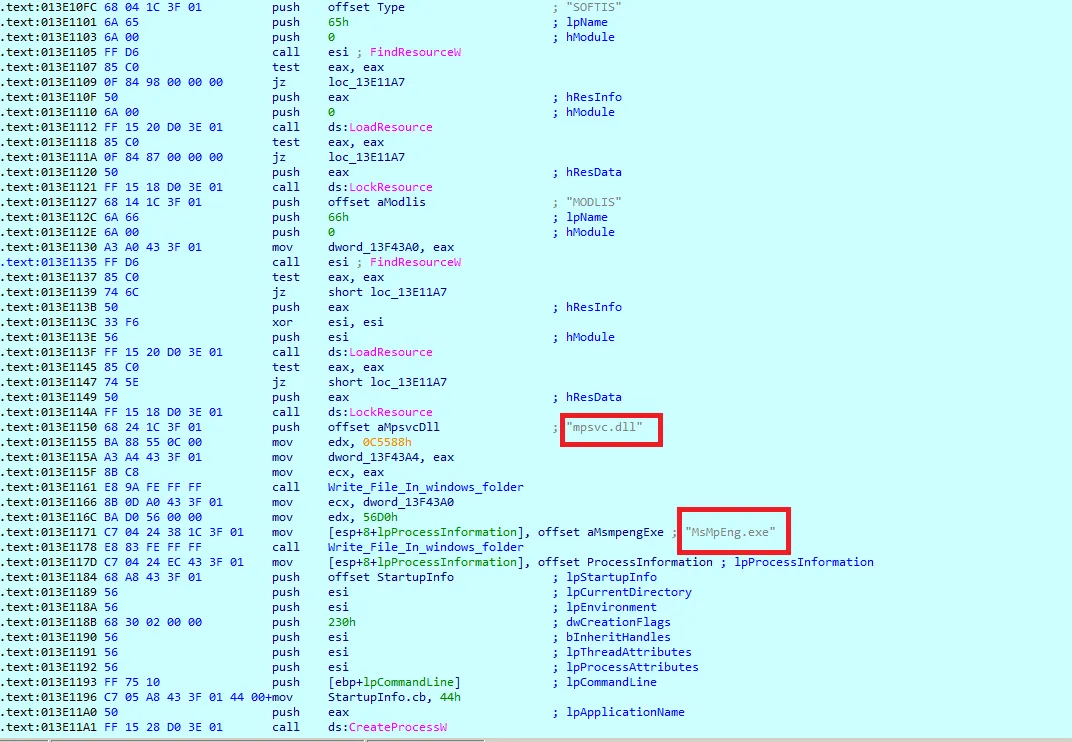
\includegraphics[width=0.8\linewidth]{rysunki/obnjdumpagenta.png}
    \caption{Miejsce w pliku binarnym \texttt{agent.exe}, w którym wywoływany jest \texttt{MsMpeng} oraz ładowany plik \texttt{.dll}. }
    \label{fig:enter-label}
\end{figure}
Innym znanym RaaS jest \foreignquote{english}{DarkSide} używany przez grupę \foreignquote{english}{CARBON SPIDER}. Do niedawna skupiał się głownie na atakach maszyn Windowsowych, niedawno rozszerzając się na systemy Linux, VMware ESXi i vCenter~\cite{darkside}. Wirus w wersji Windowsowej obchodzi zabezpieczenia kontroli użytkownika za pomocą interfejsu \texttt{CMSTPLUA COM}~\footnote{Takie obejście można dokonać programem https://github.com/tijme/cmstplua-uac-bypass}, następnie sprawdza na podstawie lokalizacji i języka systemu w celu ominięcia ataku na maszynę z jednej z byłych republik radzieckich. Program podejmuje potem następujące kroki:
\begin{enumerate}
    \item tworzy plik \texttt{LOG.<id użytkownika>.TXT} w którym przechowuje dane tymczasowe na temat progresu ataku,
    \item usuwa pliki w koszu, programy antywirusowe i zapewniające bezpieczeństwo oraz zamyka procesy blokujące mu dostęp do danych użytkownika,
    \item rozpoczyna szyfrowanie algorytmem \texttt{Salsa20} przy pomocy losowo wygenerowanego klucza macierzowego,
    \item klucz macierzowy jest szyfrowany zakodowanym na twardo kluczem RSA, a następnie łączony z zaszyfrowanym plikiem,
    \item pozostawia plik \texttt{README.<id użytkownika>.TXT} w którym wskazuje stronę ukrytą za TORem, na której ofiara ma dokonać płatność w BTC lub XMR.
\end{enumerate}
\begin{figure}[H]
    \centering
    
\includegraphics[width=0.75\linewidth]{rysunki/tapeta.png}
    \caption{W wyniku działania wirusa tapeta użytkownika zostaje zmieniona na taką, jak widać na obrazku..}
    \label{fig:enter-label}
\end{figure}
%%%%%%%%%%%%%%%%%%%%%%%%%%%%%%%%%%%%%%%%%%%%%%%%
\section{Istniejące techniki wykrywania i obrony przed ransomware}
Niezależnie od tego czy atakujący korzysta z techniki \foreignquote{english}{living off the land} lub stara się spowodować starty w możliwie najmniejszym przedziale czasowym, w przeciwdziałaniu atakom ransomware najważniejsza jest szybka reakcja. Wykrywanie ataków ransomware można osiągnąć poprzez monitorowanie nietypowych dla środowiska działań, a następnie natychmiastowe powiadomienie o nich użytkownika lub administratora. Po powiadomieniu administrator może wyizolować, a potem usunąć zagrożenie nim atak spowoduje większe straty. Dzięki wczesnej reakcji administratora i systematycznemu harmonogramowi kopii zapasowych ofiara nie musi być zdana na łaskę atakującego.
\newline
Wyróżnia się trzy główne metody wykrywania ataku: poprzez sygnaturę plików, poprzez analizę nietypowego dla systemu zachowania oraz poprzez monitorowanie ruchu sieciowego~\cite{vehabovic_ransomware_2022}.
%%%%%%%%%%%%%%%%%%%%%%%%%%%%%%%%%%%%%%%%%%%%%%%%
\subsection{Wykrywanie poprzez sygnaturę plików}
Zasada działania tego typu wykrywania jest bardzo prosta. Oprogramowanie ma pewne unikalne cechy, na podstawie których wyliczana jego sygnatura. Do tych cech należą zakodowane na twardo nazwy domen, adresy IP oraz inne identyfikatory. Typowo także wykorzystywana jest wartość funkcji skrótu dla pliku. Do użycia tego sposobu musi istnieć często aktualizowana baza danych zawierająca sygnatury wszystkich napotkanych typów ransomware. Niestety sposób ten jest ograniczony do wirusów napotkanych w przeszłości i nie jest nim możliwe wykrycie unikalnego zagrożenia. Głównie z tego powodu odchodzi się od tego rozwiązania.
\begin{figure}[H]
    \centering
    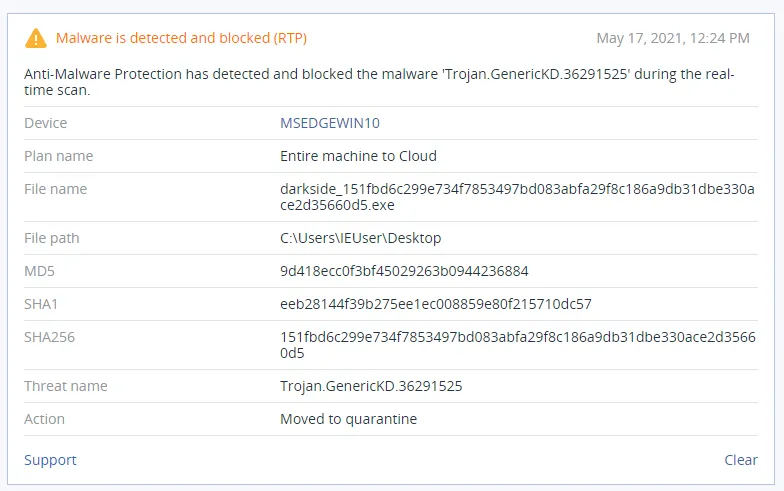
\includegraphics[width=0.75\linewidth]{rysunki/sygnatura.png}
    \caption{Tradycyjne antywirusy tak jak pokazany na obrazku Acronis, korzystają z metody wykrywania poprzez sygnaturę.}
    \label{fig:enter-label}
\end{figure}
%%%%%%%%%%%%%%%%%%%%%%%%%%%%%%%%%%%%%%%%%%%%%%%%
\subsection{Wykrywanie poprzez analizę zachowania systemu}
W przeciwieństwie do wcześniej wymienionego sposobu wykrywanie poprzez analizę zachowania system nie opiera się na sprawdzeniu treści ransomware tylko na wykryciu kroków, które podejmuje. Jest to technika, przystosowana do taktyki \foreignquote{english}{live off the land}, która stała się obiektem eksperymentów z algorytmami wykrywania wirusów opartych na sztucznej inteligencji~\cite{vehabovic_ransomware_2022}. Metoda ta polega na dopasowaniu ciągu akcji, które występują podczas ataku. Do tych akcji należą:
\begin{itemize}
    \item wykonywanie konkretnych komend powłoki systemu,
    \item pobieranie i korzystanie ze znanych i w większości otwartych programów do penetracji systemów,
    \item wykorzystywanie konkretnych zmiennych środowiskowych jako argumenty wywołań,
    \item użycie konkretnych wywołań systemowych,
    \item wykorzystywanie konkretnych obszarów systemu plików,
    \item zmiana atrybutów i właścicieli plików, folderów, punktów montowania dysków.
\end{itemize}
Jedną z najpowszechniejszych metod, używanym przez atakujących do powiadomienia ofiary o ataku i metodzie odzyskania dostępu do danych jest pozostawienie pliku tekstowego w miejscu łatwym do znalezienia np. w katalogu domowym użytkownika. Inną jest tworzenie pliku tymczasowego przechowującego stan zaawansowania ataku. Z tych powodów część metod wykrywania ransomware skupia się na wyszukiwaniu takich plików na podstawie treści, wykorzystując technikę \foreignquote{english}{bag-of-words}~\footnote{Jest to technika przedstawienia tekstu w modelu nieułożonej kolekcji słów. Wykorzystuje się ją m.in. w przetwarzaniu języka naturalnego.} w celu odnalezienia korelacji między terminami typowymi dla takich dokumentów np. \foreignquote{english}{encrypted}, \foreignquote{english}{ransom} etc.
%%%%%%%%%%%%%%%%%%%%%%%%%%%%%%%%%%%%%%%%%%%%%%%%
\subsection{Wykrywanie poprzez analizę ruchu sieciowego}
Wykrywanie poprzez analizę ruchu siecioweg polega na ograniczenia analizy behawioralnej do wąskiego zakresu zachowań systemu.
Metoda ta polega na monitorowaniu transferów danych do maszyn o nieznanych i podejrzanych adresach
oraz domenach. Zgodnie z techniką \foreignquote{english}{live off the land}, atakujący będzie chciał
możliwe zminimalizować komunikację z serwerami zewnętrznymi które mogą zostać uznane za podejrzane, mimo to 
znakomita większość narzędzi hakerskich, jest ogólnodostępna i dobrze znana w branży
cyberbezpieczeństwa i tym samym nie trudne do wykrycia~\cite{sans_secure}.  
\begin{table}[H]
    \centering
    \begin{tabular}{ll}
    \hline
    \multicolumn{1}{|l|}{Narzędzie} & \multicolumn{1}{l|}{Strona}  \\ \hline
    7zip                            & 7-zip.org                    \\
    AdFind                          & joeware.net                  \\
    Advanced IP Scanner             & advanced-ip-scanner.com      \\
    AnyDesk                         & anydesk.com                  \\
    Proces Hacker                   & processhacker.sourceforge.io \\
    rclone                          & rclone.org                   \\
    WinSCP                          & winscp.net                  
    \end{tabular}
    \caption{Tabela popularnych narzędzi używanych przez operatorów ransomware i odpowiadające im strony. Dane pochodzą ze strony: https://lots-project.com/}
\end{table}
%%%%%%%%%%%%%%%%%%%%%%%%%%%%%%%%%%%%%%%%%%%%%%%%
\section{Metody analizy statystyk systemu plików}
%%%%%%%%%%%%%%%%%%%%%%%%%%%%%%%%%%%%%%%%%%%%%%%%
\section{Podstawy działania systemów plików}
 